\section{Results}\label{sec:results}

The results proceed from engagement presence to the conditions that differentiate its depth. We first ask whether everyday human--LLM conversations contain learning-oriented engagement, distinguishing broad cognitive uptake from the highest-level constructive form. We then examine where constructive engagement is concentrated across user framing, task ecology and sustained exchange. Finally, we ask how assistant scaffolding relates to constructive engagement: first as a conversation-level condition, then through support forms, and finally through adjacent-turn temporal ordering. Because the logs contain no direct assessment of knowledge gain, engagement labels are interpreted as behavioural signatures of potential learning, and scaffolding analyses are interpreted as associations rather than causal evidence of learning effects.


% \section{Results}\label{sec:results}



% The results proceed from engagement presence to the conditions that differentiate its depth. We first ask whether everyday human--LLM conversations contain learning-oriented engagement, distinguishing broad cognitive uptake from the highest-level constructive form. We then examine where constructive engagement is concentrated across user framing, task ecology and sustained exchange. Finally, we ask how assistant scaffolding relates to constructive engagement: first as a conversation-level condition, then through support forms, and finally through adjacent-turn temporal ordering. Because the logs contain no direct assessment of knowledge gain, engagement labels are interpreted as behavioural signatures of potential learning, and scaffolding analyses are interpreted as associations rather than causal evidence of learning effects.



% \subsection{Everyday human--LLM conversations contain learning-oriented engagement}



% Across the four dataset-by-task settings, 30.3\% of user turns showed cognitive engagement, 4.9\% reached constructive engagement, and emotional engagement was rare, appearing in only 0.62\% of user turns (Table~\ref{tab:dataset_overview}). This establishes the first descriptive pattern: everyday human--LLM interaction contains observable learning-oriented engagement, but that engagement is primarily cognitive rather than affective, and only a smaller subset reaches the more generative constructive form. In other words, users often did more than simply request or receive task output, but the depth of their engagement varied.






% Figure~\ref{fig:engagement_ecology}a decomposes cognitively engaged turns into passive receipt, active uptake and constructive engagement. Active uptake accounted for 70.8\% to 86.3\% of cognitively engaged turns across the four dataset-by-task settings, constructive engagement for 12.6\% to 23.5\%, and passive receipt for 1.1\% to 6.9\%. Thus, learning-oriented engagement was not a binary signal but a depth-graded pattern. Most cognitively engaged turns involved active uptake: users used, applied or followed up on the assistant's response. A smaller but stable subset involved constructive engagement, in which users elaborated, tested, revised or extended ideas. This distinction matters for the rest of the Results. Cognitive engagement provides the broad signal that everyday LLM use can become learning-oriented, active uptake shows that users often work with the assistant's response, and constructive engagement identifies the deepest cases of user participation that we seek to explain. The following analyses therefore focus on where this constructive form appears and which interactional conditions are associated with it.


\subsection{Everyday human--LLM conversations contain learning-oriented engagement}

Across the six WildChat, LMSYS Chat and ShareChat task settings, 31.9\% of user turns showed cognitive engagement, 4.9\% reached constructive engagement, and visible emotional expression was rare, appearing in only 0.74\% of user turns (Table~\ref{tab:dataset_overview}). This establishes the first descriptive pattern: users often engage with assistant responses in learning-oriented ways rather than merely passively acknowledging or receiving task output, while visible affective expression is limited.

% everyday human--LLM interaction contains observable learning-oriented engagement, but that engagement is primarily cognitive rather than affective, and only a smaller subset reaches the more generative constructive form. In other words, users often did more than simply request or receive task output, but the depth of their engagement varied.

Figure~\ref{fig:engagement_ecology}a decomposes cognitively engaged turns into passive receipt, active uptake and constructive engagement across the six task settings. Active uptake was the dominant form of cognitive engagement, while the highest-level constructive form made up a smaller but stable subset.
% Thus, learning-oriented engagement was not a binary signal but a depth-graded pattern. 
A majority of cognitively engaged turns involved active uptake: users used, applied or followed up on the assistant's response. A smaller but stable subset involved constructive engagement, in which users elaborated, tested, revised or extended ideas. This distinction matters for the rest of the Results. Cognitive engagement provides the broad signal that everyday LLM use can become learning-oriented, active uptake shows that users often work with the assistant's response, and constructive engagement identifies the deepest cases of user participation that we seek to explain. The following analyses therefore focus on where this constructive form appears and which interactional conditions are associated with it.



% \begin{table*}[t]
% \small
% \centering
% \caption{\textbf{Dataset and behavioural overview.} Summary statistics for the four matched settings analysed in the study. Percentages for cognitive, constructive and emotional engagement are computed over user turns; percentages for scaffolding support are computed over assistant turns.}
% \label{tab:dataset_overview}

% \setlength{\tabcolsep}{4pt}
% \renewcommand{\arraystretch}{1.1}

% \resizebox{\textwidth}{!}{%
% \begin{tabular}{lrrrrrrrr}
% \toprule
% Setting 
% & Conversations 
% & \makecell{User\\turns} 
% & \makecell{Assistant\\turns} 
% & \makecell{Intentional\\conv. (\%)} 
% & \makecell{S2 turns\\(\%)} 
% & \makecell{Cognitive\\(\%)} 
% & \makecell{Constructive\\(\%)} 
% & \makecell{Emotional\\(\%)} \\
% \midrule
% WildChat coding  & 31,878 & 124,073 & 124,623 & 37.13 & 51.03 & 50.21 & 9.23 & 0.95 \\
% WildChat writing & 39,534 & 163,705 & 164,824 & 25.80 & 23.53 & 16.34 & 2.22 & 0.57 \\
% Copilot coding   & 31,879 & 127,435 & 125,610 & 44.59 & 49.50 & 48.11 & 6.05 & 0.76 \\
% Copilot writing  & 39,534 & 148,401 & 146,641 & 36.98 & 41.00 & 13.88 & 3.26 & 0.30 \\
% \midrule
% Total / pooled   & 142,825 & 563,614 & 561,698 & -- & 40.00 & 30.3 & 4.9 & 0.62 \\
% \bottomrule
% \end{tabular}%
% }
% \end{table*}

\begin{table*}[t]
\small
\centering
\caption{
\textbf{Dataset and behavioural overview.}
Summary statistics for the two WildChat task settings analysed in the study. Constructive engagement is reported as the stricter depth level within cognitive engagement and serves as the focal user-side outcome in subsequent analyses.
}
\label{tab:dataset_overview}

\setlength{\tabcolsep}{4pt}
\renewcommand{\arraystretch}{1.1}

\resizebox{\textwidth}{!}{%
\begin{tabular}{lrrrccccc}
\toprule
& \multicolumn{3}{c}{Sample size}
& \multicolumn{1}{c}{User framing}
& \multicolumn{1}{c}{Assistant support}
& \multicolumn{2}{c}{Cognitive engagement}
& \multicolumn{1}{c}{Emotional engagement} \\
\cmidrule(lr){2-4}
\cmidrule(lr){5-5}
\cmidrule(lr){6-6}
\cmidrule(lr){7-8}
\cmidrule(lr){9-9}
Setting 
& Conversations 
& \makecell{User\\turns} 
& \makecell{Assistant\\turns} 
& \makecell{Intentional\\conv. (\%)} 
& \makecell{Scaffolded\\turns (\%)} 
& \makecell{Overall\\(\%)} 
& \makecell{Constructive\\level (\%)} 
& \makecell{Emotional\\(\%)} \\
\midrule
WildChat coding  & 31,878 & 124,073 & 124,623 & 37.13 & 51.03 & 50.21 & 9.23 & 0.95 \\
WildChat writing & 39,534 & 163,705 & 164,824 & 25.80 & 23.53 & 16.34 & 2.22 & 0.57 \\
\midrule
Total / pooled   & 71,412 & 287,778 & 289,447 & 30.86 & 35.37 & 30.9 & 5.2 & 0.73 \\
\bottomrule
\end{tabular}%
}

\vspace{2mm}
\begin{minipage}{0.98\textwidth}
\footnotesize
\textit{Note.} Percentages for cognitive, constructive and emotional engagement are computed over user turns; percentages for scaffolded support are computed over assistant turns. The constructive-level column reports the share of all user turns that reached the constructive depth level within cognitive engagement. Figure~\ref{fig:engagement_ecology}a reports the composition of passive, active and constructive uptake among cognitively engaged turns.
\end{minipage}
\end{table*}


% \subsection{Constructive engagement is shaped by user framing, task ecology and interaction depth}


% %%%%%%%%%%%%%%%%%%%%%%%%%%%%%%%%%%%%%%%%%%
% Having established that everyday human--LLM conversations contain learning-oriented engagement, we next examined where its constructive form was concentrated. User framing provided the first contrast (Fig.~\ref{fig:engagement_ecology}b). Across all four dataset-by-task settings, conversations explicitly oriented toward learning or exploration showed higher engagement than conversations without such framing. Cognitive engagement increased from 6.4--33.2\% in unintentional conversations to 26.0--76.6\% in intentional conversations, and constructive engagement increased from 1.5--5.7\% to 5.2--13.1\%. Explicit learning or exploratory framing therefore amplified constructive engagement, but did not create it from zero: even task-oriented conversations without explicit learning intent contained constructive participation.

% Task ecology provided a second source of variation. In the two everyday task ecologies sampled here, coding-oriented conversations showed higher engagement than writing-oriented conversations in both datasets. Cognitive engagement was 48.1--50.2\% in coding conversations, compared with 13.9--16.3\% in writing conversations; constructive engagement was 6.1--9.2\% in coding and 2.2--3.3\% in writing. Importantly, this contrast was not reducible to explicit learning framing: in both datasets, unintentional coding conversations showed higher cognitive engagement than intentional writing conversations. This pattern suggests that task ecology was not merely a backdrop for explicit learning intent; it shaped the baseline opportunities for users to ask questions, test assumptions, refine solutions and extend ideas. One plausible reason is that coding tasks often make uncertainty and failure externally visible through errors, constraints and executable tests, whereas writing tasks may more often be resolved through drafting, editing or applying a proposed revision without requiring users to articulate the underlying rationale~\ToCite{}.


% Interaction depth provided a third lens on where constructive participation surfaced (Fig.~\ref{fig:engagement_ecology}c). Across all four dataset-by-task settings, the probability that a conversation contained at least one constructive user turn increased monotonically with behavioural depth, from 0.060--0.151 in 2--3-turn conversations to 0.150--0.463 in conversations with seven or more turns. The gradient was steepest in coding-oriented conversations, but the same direction appeared in writing-oriented conversations as well. Because this measure captures whether a constructive turn occurred at least once in a conversation, longer exchanges naturally provide more opportunities for such turns to appear and may also reflect more complex tasks or more engaged users. We therefore do not interpret depth as evidence that turns accumulate into learning progress by themselves. The substantive point is instead that constructive engagement is most visible when everyday LLM use moves beyond one-off answer delivery and becomes a sustained exchange in which users return to, interrogate and reshape the assistant's response.



% Together, these results show that constructive engagement is ecological. It is amplified by explicit learning framing, varies across task ecologies and concentrates in sustained exchanges. This motivates the next step of the analysis: asking whether assistant scaffolding is one interactional condition associated with richer constructive participation.



\subsection{Constructive engagement varies systematically with user framing, task ecology and interaction depth}

Having established that everyday human--LLM conversations contain learning-oriented engagement, we next examined where its constructive form was concentrated. User framing provided the first contrast (Fig.~\ref{fig:engagement_ecology}b). Across the six main settings, conversations explicitly oriented toward learning or exploration showed higher engagement than conversations without such framing. Importantly, both explicitly learning-oriented and more task-oriented conversations contained constructive participation, indicating that informal learning-relevant engagement was not confined to interactions that announced themselves as learning episodes.
% Explicit learning amplified constructive engagement. even task-oriented conversations without explicit learning intent contained constructive participation.

Task ecology provided a second source of variation. In the two everyday task ecologies sampled here, coding-oriented conversations showed higher constructive engagement than writing-oriented conversations across WildChat, LMSYS and ShareChat. Cognitive engagement was 45.00--50.21\% in coding conversations, compared with 15.30--33.05\% in writing conversations; constructive engagement was 5.43--15.17\% in coding and 1.53--5.18\% in writing. 
% Importantly, this contrast was not reducible to explicit learning framing: unintentional coding conversations showed higher cognitive engagement than intentional writing conversations. 
% This pattern suggests that task ecology shaped the baseline opportunities for users to ask questions, test assumptions, refine solutions and extend ideas. 
The LMSYS coding setting illustrates why broad cognitive uptake and deeper constructive engagement should remain separate outcomes: because LMSYS Chat reflects an earlier public-demo and Chatbot Arena period~\cite{zheng2023lmsyschat1m}, many coding exchanges involved active repair questions, added constraints and requests for another direct coding step, which can raise active uptake without producing the same level of constructive elaboration.
One plausible reason for a higher engagement rate of coding tasks is that they often make uncertainty and failure externally visible through errors, constraints and executable tests, whereas writing tasks may more often be resolved through drafting, editing or applying a proposed revision without requiring users to articulate the underlying rationale~\cite{keuning2018systematic,flower1981cognitive,sommers1980revision}.
This pattern suggests that task ecology was associated with baseline opportunities for users to ask questions, test assumptions, refine solutions and extend ideas. 

% Interaction depth provided a third lens on where constructive participation surfaced (Fig.~\ref{fig:engagement_ecology}c). Across the two WildChat task settings, the probability that a conversation contained at least one constructive user turn increased monotonically with behavioural depth, from 0.060--0.151 in 2--3-turn conversations to 0.150--0.463 in conversations with seven or more turns. The gradient was steeper in coding-oriented conversations, but the same direction appeared in writing-oriented conversations as well. Because this measure captures whether a constructive turn occurred at least once in a conversation, longer exchanges naturally provide more opportunities for such turns to appear and may also reflect more complex tasks or more engaged users. We therefore do not interpret depth as evidence that turns accumulate into learning progress by themselves. The substantive point is instead that constructive engagement is most visible when everyday LLM use moves beyond one-off answer delivery and becomes a sustained exchange in which users return to, interrogate and reshape the assistant's response.

Interaction depth provided a third lens on where constructive participation surfaced (Fig.~\ref{fig:engagement_ecology}c). Across the six main settings, the probability that a conversation contained at least one constructive user turn increased with behavioural depth. Because this measure asks whether a rare event occurred at least once, part of the gradient is mechanical: longer conversations provide more opportunities to observe a constructive turn. We therefore interpret Fig.~\ref{fig:engagement_ecology}c as a descriptive visibility pattern, not as evidence that length itself produces deeper engagement. A grouped-binomial rate sensitivity, modelling constructive user-turn counts out of total user turns with user framing, task ecology, length bucket and dataset fixed effects, showed a much smaller but still positive length association (OR=1.13 for 4--6 user turns; OR=1.06 for 7+ user turns; Supplementary Table~\ref{tab:constructive_rate_context_logit}). The substantive point is that constructive engagement is most visible when everyday LLM use becomes a sustained exchange rather than a one-off request for an answer.
% Interaction depth is therefore best understood as an opportunity structure for constructive participation: it marks the conversational conditions under which users can continue working with ideas.

Together, these results show that constructive engagement is ecological. It is amplified by intentional user framing, varies across task ecologies and is most visible in sustained exchanges. A simple conversation-level logistic check showed the same directional organization after including user framing, task ecology, conversation-length bucket and dataset fixed effects (Supplementary Table~\ref{tab:constructive_context_logit}), and the constructive-rate sensitivity shows that the length pattern is not only an opportunity-count artifact.
% This motivates the next step of the analysis: asking whether assistant scaffolding is one interactional condition associated with richer constructive participation.



\begin{figure*}[t]
    \centering
    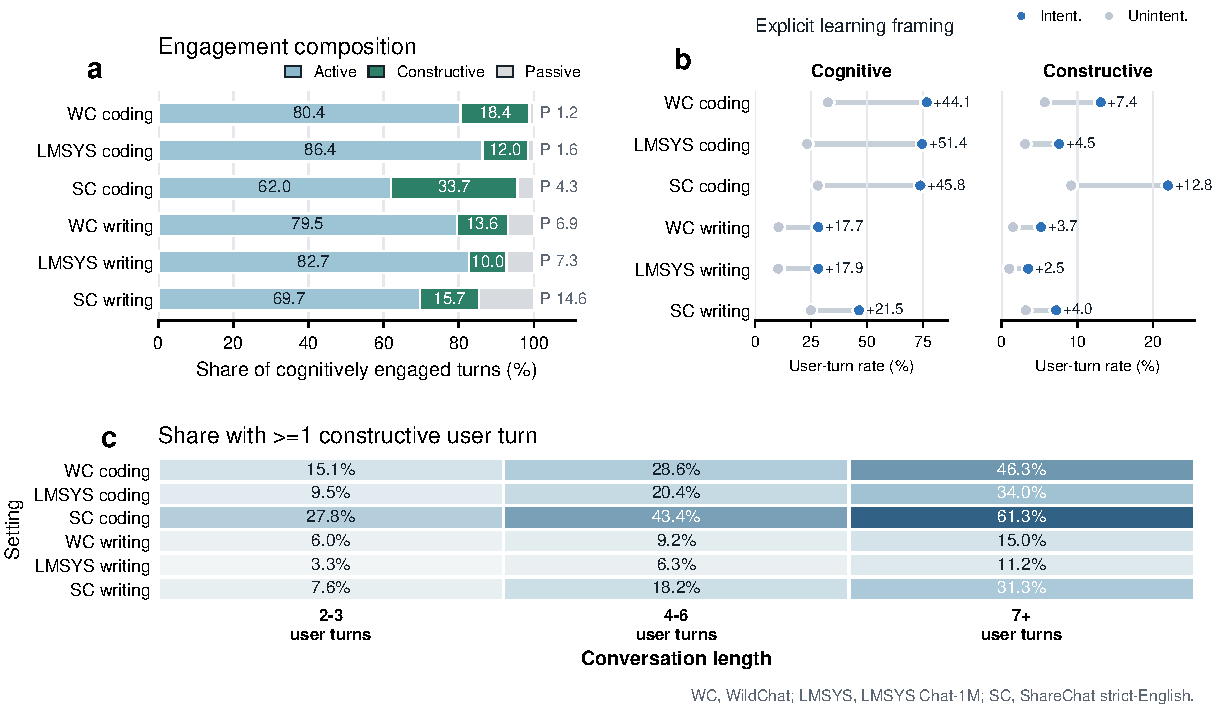
\includegraphics[width=\textwidth]{figures/fig_engagement_ecology_compact_final.pdf}
    \caption{
    \textbf{Learning-oriented engagement varies by engagement form, user framing and conversation length.}
    \textbf{a,} Composition of cognitively engaged user turns by active, constructive and passive levels across the six task settings.
    \textbf{b,} Cognitive and constructive engagement rates in conversations with intentional versus unintentional user framing.
    \textbf{c,} Share of conversations with at least one constructive user turn by conversation-length bucket.
    Panel a uses cognitively engaged turns as the denominator; panel b reports percentages of user turns; panel c reports conversation-level shares. WC, WildChat; LMSYS, LMSYS Chat; SC, ShareChat.
    }
    \label{fig:engagement_ecology}
\end{figure*}



\subsection{Scaffolded conversations show richer constructive participation}

After characterizing user-side conditions such as user framing and task ecology, we next examined how assistant behaviour was associated with richer constructive participation through scaffolding, a canonical way that teachers support engagement.
At the conversation level, conversations containing at least one scaffolded assistant turn had higher constructive ratios than conversations without scaffolded support in all six task settings (Fig.~\ref{fig:s2_conversation_association}a). Using the same turn-weighted estimator in Fig.~\ref{fig:s2_conversation_association}a, Table~\ref{tab:support_engagement_summary} and Supplementary Table~\ref{tab:key_contrast_significance}, these raw constructive-ratio differences ranged from +0.99 to +7.34 percentage points across WildChat, LMSYS and ShareChat, and scaffolded conversations also showed greater post-first-response depth in every setting (+1.43 to +3.38 turns; Fig.~\ref{fig:s2_conversation_association}d). All six constructive-ratio contrasts and all six depth contrasts were statistically distinguishable from zero in conversation-level bootstrap tests ($p<.001$; Supplementary Table~\ref{tab:key_contrast_significance}). These descriptive contrasts show that scaffolding co-occurred with both more constructive participation and more sustained exchange; the percentage-point differences are reported as effect sizes. Because S2 presence is itself more observable in longer exchanges, depth differences are interpreted as descriptive co-occurrence rather than evidence that scaffolding lengthened conversations.

The association remained positive after adjusting for observed user framing, task ecology and conversation-level context in covariate-adjusted models. Across the six settings, Poisson count ratios for constructive-turn counts ranged from 1.569 to 2.491, and logistic odds ratios for whether a conversation contained at least one constructive turn ranged from 1.437 to 2.140 (Fig.~\ref{fig:s2_conversation_association}b). These count ratios and odds ratios are reported as model-based effect-size estimates, indicating that scaffolded support remained associated with higher constructive participation after observed-covariate adjustment. A setting-specific offset-rate sensitivity, using \texttt{log(user\_turns)} as the exposure offset and quasi-Poisson scaled standard errors, preserved positive \texttt{has\_S2} associations in all six settings (rate ratios 1.356--1.703; all $p<.001$; Supplementary Table~\ref{tab:fig3_offset_rate_sensitivity}).





\begin{figure*}[t]
  \centering
  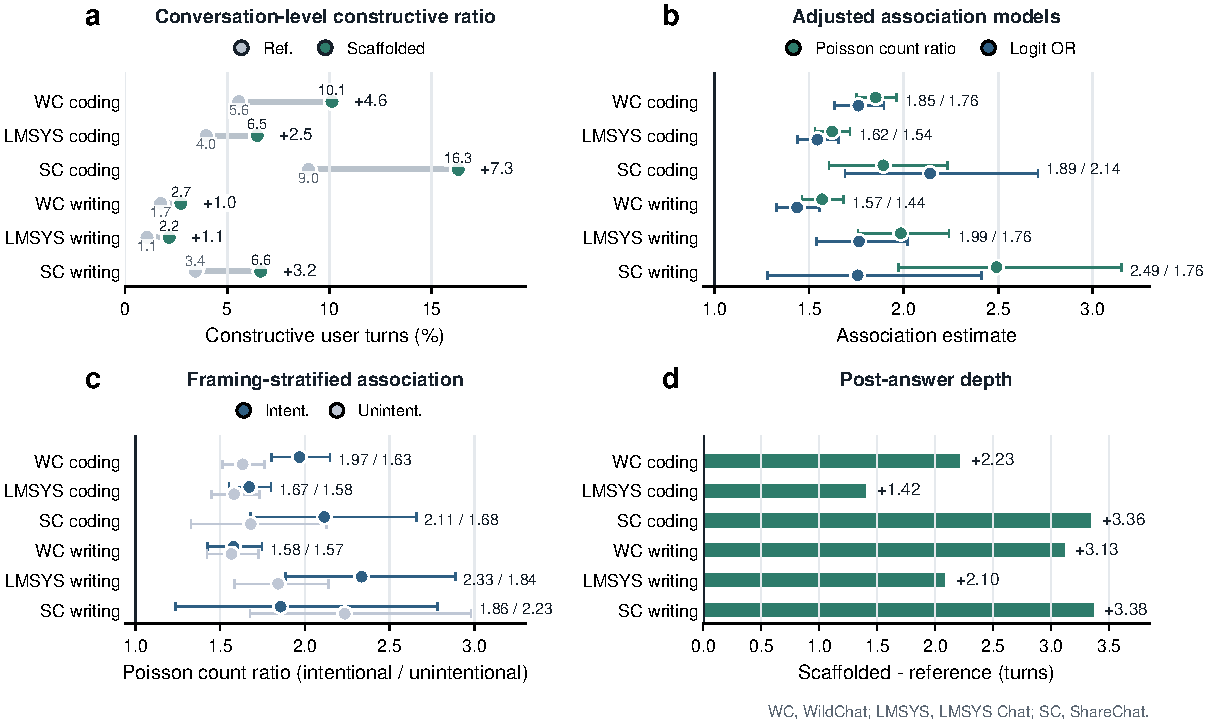
\includegraphics[width=\linewidth]{figures/fig_support_association_wild_lmsys_with_ci.pdf}
    \caption{
    \textbf{Scaffolded conversations are associated with richer constructive participation across the three corpora.}
    \textbf{a,} Turn-weighted constructive user-turn ratios in conversations with versus without scaffolded support.
    \textbf{b,} Covariate-adjusted associations between scaffolded-support presence and constructive participation, reported as Poisson count ratios and logistic odds ratios.
    \textbf{c,} Poisson count ratios for scaffolded-support presence stratified by intentional versus unintentional user framing.
    \textbf{d,} Difference in post-answer interaction depth after the first assistant response.
    Numbers indicate scaffolded-minus-reference differences, except panels b and c, which report model estimates. Error bars in panels b and c show model-based 95\% confidence intervals; Poisson overdispersion and offset-rate sensitivities are reported in Methods and the Appendix.
    }
  \label{fig:s2_conversation_association}
\end{figure*}



% \begin{table*}[t]
% \small
% \centering
% \caption{\textbf{Summary of key support--engagement effects across the four matched settings.} Constructive-ratio contrasts compare conversations with versus without scaffolding support. Adjusted models report the association of having scaffolding support with constructive-turn count (Poisson rate ratio) and with having at least one constructive turn (logit odds ratio). Adjacent-turn lift is the difference in the probability that the next user turn is constructive after scaffolded versus direct-response assistant turns.}
% \label{tab:key_effects}

% \setlength{\tabcolsep}{4pt}
% \renewcommand{\arraystretch}{1.1}

% \resizebox{\textwidth}{!}{%
% \begin{tabular}{lrrrrrrr}
% \toprule
% Setting 
% & \makecell{Constructive ratio\\Has S2 / No S2}
% & \makecell{Difference\\(pp)}
% & \makecell{Depth diff.\\(turns)}
% & \makecell{Poisson\\RR}
% & \makecell{Logit\\OR}
% & \makecell{Adjacent lift\\(pp)}
% & \makecell{Around first S2\\diff.} \\
% \midrule
% WildChat coding  & 0.094 / 0.055 & +3.9 & +2.23 & 1.852 & 1.761 & +2.68 & +0.014 \\
% WildChat writing & 0.032 / 0.020 & +1.2 & +3.13 & 1.569 & 1.437 & +1.13 & -0.042 \\
% Copilot coding   & 0.062 / 0.035 & +2.7 & +2.63 & 1.870 & 1.736 & +1.65 & -0.003 \\
% Copilot writing  & 0.037 / 0.026 & +1.1 & +1.61 & 1.240 & 1.251 & +0.01 & -0.039 \\
% \bottomrule
% \end{tabular}%
% }
% \end{table*}

\begin{table*}[t]
\small
\centering
\caption{
\textbf{Summary of key support--engagement associations in WildChat.}
Constructive-ratio contrasts compare conversations with versus without scaffolded support. Adjusted models report the association of scaffolded-support presence with constructive-turn count (Poisson rate ratio) and with having at least one constructive turn (logit odds ratio). Adjacent-turn lift is the difference in the probability that the next user turn is constructive after scaffolded versus non-scaffolded reference assistant turns.
}
\label{tab:support_engagement_summary}

\setlength{\tabcolsep}{5pt}
\renewcommand{\arraystretch}{1.1}

\resizebox{\textwidth}{!}{%
\begin{tabular}{lrrrrrrr}
\toprule
Setting 
& \makecell{Constructive ratio\\Has S2 / No S2}
& \makecell{Difference\\(pp)}
& \makecell{Depth diff.\\(turns)}
& \makecell{Poisson\\RR}
& \makecell{Logit\\OR}
& \makecell{Adjacent lift\\(pp)}
& \makecell{Around first S2\\diff.} \\
\midrule
WildChat coding  & 0.094 / 0.055 & +3.9 & +2.23 & 1.852 & 1.761 & +2.68 & +0.014 \\
WildChat writing & 0.032 / 0.020 & +1.2 & +3.13 & 1.569 & 1.437 & +1.13 & -0.042 \\
\bottomrule
\end{tabular}%
}
\end{table*}



% \subsection{Support forms distinguish broad cognitive uptake from constructive engagement}\label{subsec:support_form}

% The conversation-level association did not imply that all forms of scaffolding carried the same engagement signal. We therefore decomposed scaffolded support into the six support forms in the annotation scheme (M1--M6) and compared scaffolded conversations containing each form with scaffolded conversations that did not contain that form, stratified by intentional versus unintentional learning orientation. Because support-form labels were not mutually exclusive, these contrasts are descriptive associations rather than effects of isolated instructional moves. Even with this constraint, the pattern differentiated broad cognitive uptake from constructive engagement (Fig.~\ref{fig:support_form_supply}a).


% The overall cognitive-engagement panel shows how support forms drew users into learning-oriented participation. Feedback and hinting were more strongly associated with cognitive engagement in unintentional conversations than in intentional conversations (M1: +16.7 versus +1.7 percentage points; M2: +14.2 versus +8.4 points). This pattern suggests that evaluative feedback and partial cues may be especially useful for pulling otherwise task-oriented exchanges into cognitive work. Explanation and modelling, by contrast, showed larger cognitive-engagement contrasts in intentionally framed conversations (M4: +27.0 versus +16.7 points; M5: +11.4 versus +9.9 points), consistent with these forms aligning with users who are already seeking understanding. Instructing and questioning showed a different profile: instructing was negatively associated with cognitive engagement in both framing groups, and questioning was negative in intentional conversations and near zero in unintentional conversations. A plausible interactional explanation is that detailed instructions can make the next step executable without requiring users to articulate or revise their understanding, while questions in everyday assistant use may often function as clarification requests rather than designed Socratic prompts.


% The constructive-engagement panel sharpened this distinction by separating broad cognitive uptake from more generative participation. Feedback-like support showed the strongest constructive-engagement contrast, especially in intentionally framed conversations (M1: +12.7 versus +5.7 percentage points). This is notable because feedback did not show the same pattern for overall cognitive engagement in intentional conversations, suggesting that its contribution is not simply to increase participation in general. Rather, feedback may be especially aligned with constructive engagement because it responds to a user's prior attempt and creates an occasion for revision, evaluation or extension. Explanation also showed positive constructive-engagement contrasts (M4: +6.0 versus +3.1 points), consistent with the idea that making mechanisms visible can support users in elaborating or testing their understanding. Hinting and modelling were positive but smaller, suggesting that partial cues and examples may support progress without always eliciting visible elaboration. By contrast, instructing and questioning were associated with lower constructive engagement in both framing groups, with stronger negative contrasts in intentionally framed conversations (M3: -4.9 versus -1.2 points; M6: -2.4 versus -0.7 points). Thus, the support forms most aligned with constructive engagement were those that preserved room for users to evaluate, revise and extend ideas, rather than those that primarily prescribed the next step or shifted the exchange into clarification.







\subsection{Support forms differentiate constructive engagement}\label{subsec:support_form}

% The conversation-level association did not imply that all forms of scaffolding carried the same engagement signal. We therefore decomposed scaffolded support into the six support forms in the annotation scheme (M1--M6) and compared scaffolded conversations containing each form with scaffolded conversations that did not contain that form, stratified by intentional versus unintentional learning orientation. Because support-form labels were not mutually exclusive, these contrasts are descriptive associations rather than effects of isolated instructional moves. Even with this constraint, the pattern differentiated broad cognitive uptake from constructive engagement (Fig.~\ref{fig:support_form_supply}a).

Education theory treats scaffolding as a family of support moves rather than a single uniform intervention.
We next examined how different forms of scaffolded support were associated with users' constructive engagement. 
We decomposed scaffolded support into the six support forms in the annotation scheme (M1--M6) and, among scaffolded conversations, compared conversations containing each form with scaffolded conversations without that form (Fig.~\ref{fig:support_form_supply}a). Because support-form labels were non-mutually exclusive, these estimates describe form-level associations rather than effects of isolated instructional moves.
% Because multiple support forms can co-occur in the same conversation, each contrast should be read as a descriptive support-form association. This analysis differentiated broad cognitive uptake from the highest-level constructive form of engagement (Fig.~\ref{fig:support_form_supply}a).



The form-level pattern was sharper than the binary distinction between scaffolded and non-scaffolded support. When stratified by user framing, feedback-like support showed the largest constructive-engagement contrast in both intentional and unintentional conversations, with a stronger association under intentional framing (+14.7 versus +6.7 percentage points; framing difference, +8.0 points; Fig.~\ref{fig:support_form_supply}a). Explanation showed the same direction (+6.7 versus +3.0 points; framing difference, +3.6 points), whereas instructing and questioning were lower, especially in intentionally framed conversations. Task-stratified estimates provided a complementary check (Fig.~\ref{fig:support_form_supply}b): feedback and explanation were positive in both coding- and writing-oriented ecologies, while instructing, modelling and questioning varied more strongly by task. This pattern suggests that the forms most aligned with constructive participation were those that responded to a user's prior attempt or made mechanisms available for inspection, while more directive, example-based or clarification-oriented moves depended more strongly on the surrounding task ecology. Thus, after the conversation-level association in Section~2.3, the finer drill-down is not that all scaffolding is equally useful, but that support form shapes whether scaffolding leaves a productive role for the user in the work of understanding.



% Assistant support-intent distinctions were less discriminating. Most scaffolded support in WildChat was cognitively oriented, whereas metacognitive and emotional support were much rarer. This reinforces the central role of support form---how support was delivered---rather than broad intent category.




\begin{figure*}[t]
  \centering
  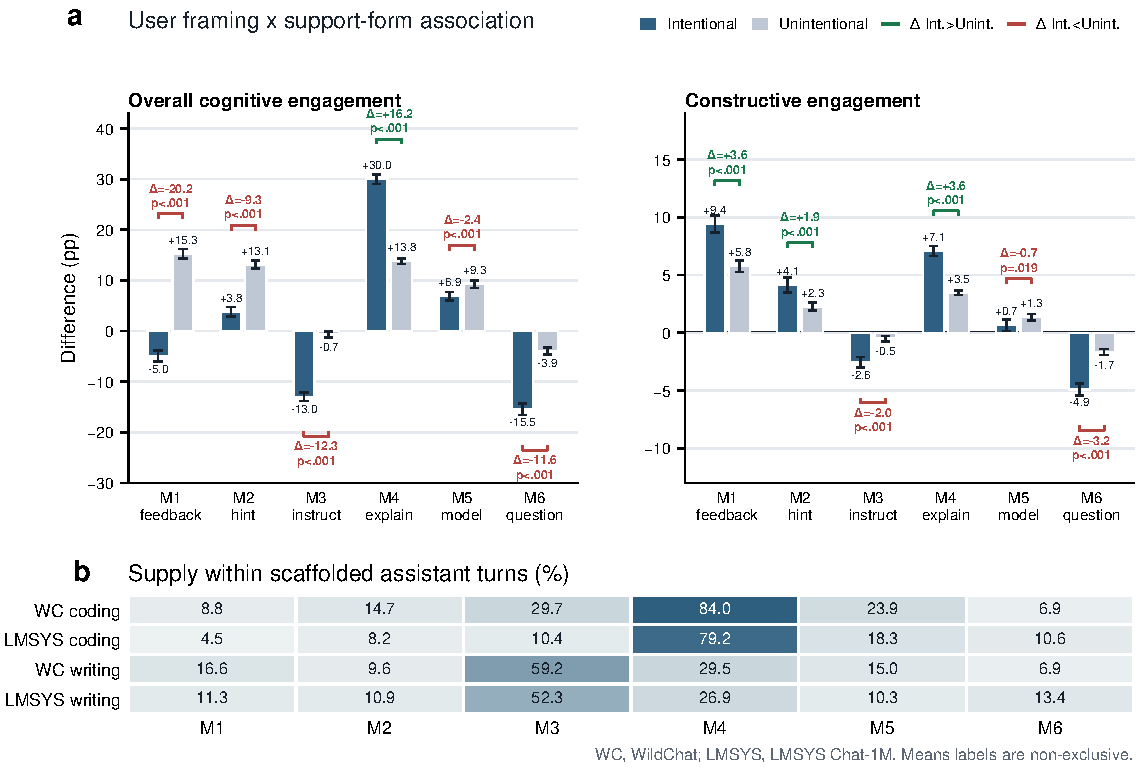
\includegraphics[width=\linewidth]{figures/fig_support_form_supply_compact_final_v2.pdf}
    \caption{
    \textbf{Support form and support supply differentiate scaffolded interaction.}
    \textbf{a,} Constructive-engagement differences associated with each support form among scaffolded conversations, stratified by intentional versus unintentional user framing.
    \textbf{b,} The same support-form contrasts stratified by coding- versus writing-oriented task ecology.
    \textbf{c,} Percentage of scaffolded assistant turns containing each support form by task setting. In panels a and b, bars are turn-weighted constructive user-turn ratio differences, comparing scaffolded conversations containing a support form with scaffolded conversations without that form; error bars show 95\% confidence intervals, and bracket annotations show between-stratum differences and Benjamini--Hochberg FDR-adjusted q values within each panel family. Support-form labels correspond to M1--M6 and are not mutually exclusive, so rows do not sum to 100\%.
    }
  \label{fig:support_form_supply}
\end{figure*}


% Together, these results show why scaffolding presence alone is too coarse to characterize learning-oriented human--LLM interaction. Scaffolded support was associated with richer constructive participation at the conversation level, but that association was carried unevenly by support form, user framing and task-specific support supply. The implication is not that systems should simply provide more scaffolding, but that learning-oriented support needs to be matched to the user's current framing and the task ecology: feedback and explanation may sustain users who are already working with ideas, whereas more directive forms may complete the task without eliciting further elaboration.


% Support supply made these form-level signatures consequential for task ecology (Fig.~\ref{fig:support_form_supply}b). Coding-oriented scaffolded turns were dominated by explanation, with M4 appearing in 84.0\% of scaffolded WildChat coding turns. Writing-oriented scaffolded turns were dominated by instructing, with M3 appearing in 59.2\% of scaffolded WildChat writing turns. Users in different task settings therefore did not merely receive more or less scaffolding; they encountered different mixtures of support. In the sampled coding ecology, scaffolded support more often took the form of explanation, which was aligned with constructive sense-making. In the sampled writing ecology, scaffolded support more often took the form of instruction, which may support task completion but was less aligned with visible constructive elaboration.

% Together, these results show why scaffolding presence alone is too coarse to characterize learning-oriented human--LLM interaction. Scaffolded support was associated with richer constructive participation at the conversation level, but that association was carried unevenly by support form, user framing and task-specific support supply. The implication is not that systems should simply provide more scaffolding, but that learning-oriented support needs to be matched to the user's current framing and the task ecology: feedback and explanation may sustain users who are already working with ideas, whereas more directive forms may complete the task without eliciting further elaboration.


Assistant support-intent labels added little separation because most scaffolded support was cognitively oriented, while metacognitive and affective intent labels were much less common (Supplementary Table~\ref{tab:support_intent_summary}). The more informative distinction was therefore how support was delivered. Figure~\ref{fig:support_form_supply}c situates this form-level pattern within task ecology: explanation dominated scaffolded coding turns across the three corpora, whereas writing-oriented support supply was more mixed and more often included instructing, explanation or questioning forms.

Together, these results show why scaffolding presence alone is too coarse to characterize learning-oriented human--LLM interaction. Scaffolded support was associated with richer constructive participation at the conversation level, but that association was carried unevenly by support form and task-specific support supply. The implication is not that systems should simply provide more scaffolding: feedback and explanation may sustain users who are already working with ideas, whereas more directive forms may complete the task without eliciting further elaboration.





% \subsection{Support and constructive engagement are locally, not cumulatively, coupled}

\subsection{Support--engagement coupling is local and state-dependent}

The preceding analyses narrowed the support result: scaffolded conversations were more constructive overall, but the association depended on support form. We finally asked whether this pattern was visible in turn ordering. If scaffolding is part of an interactional process, its clearest signal should appear locally, in how an assistant responds to the user's current state and how the next user turn continues the exchange.

\begin{figure}[!htbp]
  \centering

  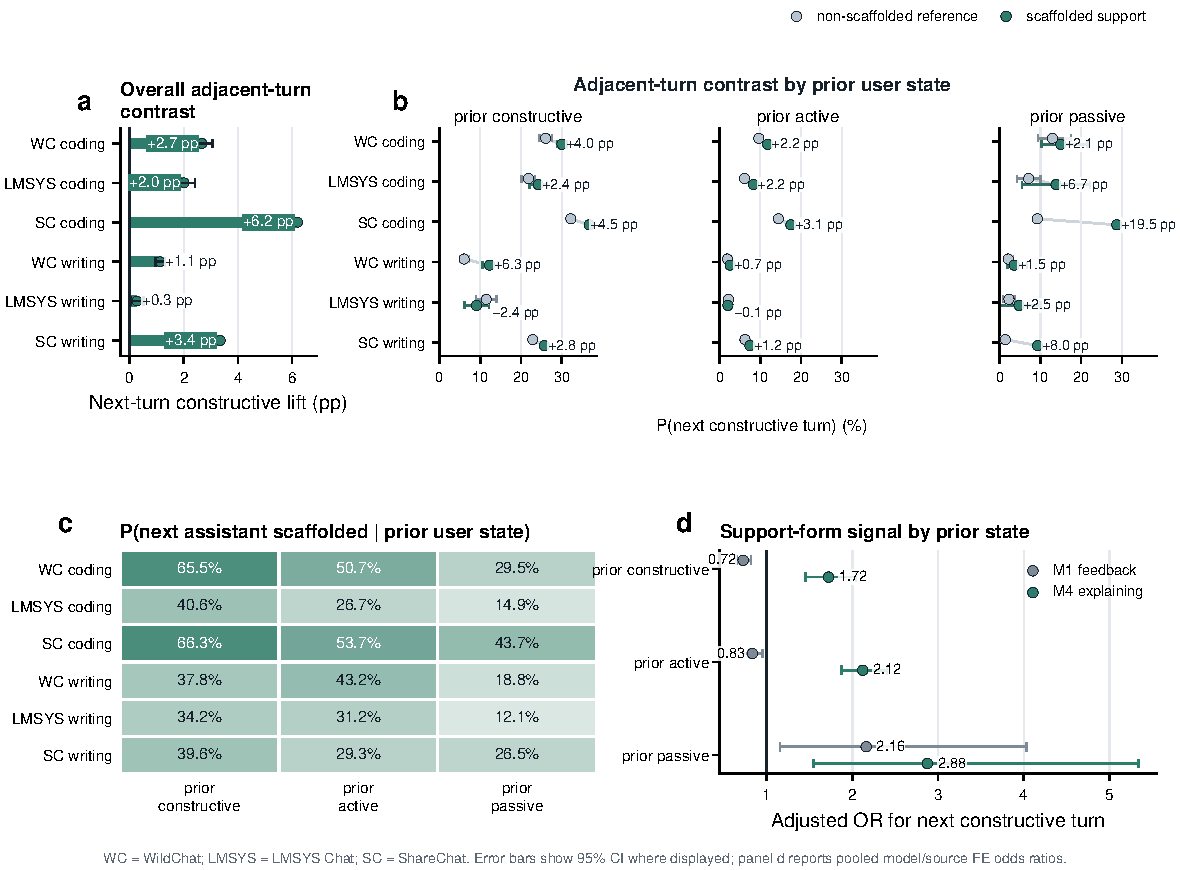
\includegraphics[width=\textwidth]{figures/fig_temporal_coupling_scale_compact_final_v5.pdf}
    \caption{
    \textbf{Support--engagement coupling is local and state-dependent across the three corpora.}
    \textbf{a,} Next-turn constructive lift after scaffolded versus non-scaffolded reference assistant turns.
    \textbf{b,} Probability of a constructive next user turn by prior user state and support condition; annotations show scaffolded-minus-reference differences.
    \textbf{c,} Probability that the next assistant turn contains scaffolded support by prior user state.
    \textbf{d,} Pooled model/source fixed-effect odds ratios for focal support forms within prior user states; M1 feedback and M4 explaining are shown because Section~2.4 identified them as the central positive conversation-level forms, and the full M1--M6 interaction table is reported in Supplementary Table~\ref{tab:prior_state_support_form_interactions}.
    Error bars show 95\% confidence intervals where displayed. Panel d reports adjacent-turn logistic models with conversation-cluster robust standard errors. WC, WildChat; LMSYS, LMSYS Chat; SC, ShareChat.
    }
  \label{fig:temporal_coupling}
\end{figure}

At this adjacent-turn scale, scaffolded assistant turns were more likely than non-scaffolded reference turns to be followed by constructive engagement in all six task settings (Fig.~\ref{fig:temporal_coupling}a). The lift was positive in each setting, ranging from +0.27 to +6.21 percentage points. Five of the six adjacent-turn lifts were statistically distinguishable from zero in conversation-cluster bootstrap tests; LMSYS writing was positive but weaker and did not cross the conventional .05 threshold (+0.27 percentage points, $p=.061$; Supplementary Table~\ref{tab:key_contrast_significance}). Thus, the temporal evidence supports a local coupling claim: scaffolded support was followed by more constructive next-turn participation, but the magnitude of that coupling varied across settings.

The local pattern was not simply a one-way effect of support on an otherwise stable user. It depended on the user's immediately preceding state. State-conditioned contrasts were generally positive but varied in size across prior constructive, active and passive turns (Fig.~\ref{fig:temporal_coupling}b). The reverse sequence showed the same contingency: assistant scaffolding was more likely after constructive or active user turns than after passive turns, especially in coding-oriented conversations (Fig.~\ref{fig:temporal_coupling}c). This bidirectional ordering suggests a coupled process in which constructive and active user turns were more often followed by scaffolded support, and scaffolded support was then associated with further constructive engagement in the next turn.

The support-form analysis also carried into the local model, but with an important refinement. Integrated adjacent-turn regressions showed that scaffolding features still added substantial signal after user state, task/framing, turn position and model/source fixed effects were included (full scaffolding block LR $\chi^2_7=1337.5$, $p<.001$; Supplementary Table~\ref{tab:integrated_scaffolding_block_tests}). Adding prior-state $\times$ support-form interactions further improved fit (pooled model/source fixed effects: LR $\chi^2_{18}=300.2$, $p<.001$; Supplementary Table~\ref{tab:prior_state_support_form_interactions}). Figure~\ref{fig:temporal_coupling}d displays M1 feedback and M4 explaining as focal forms because they were the central positive conversation-level forms in Section~2.4; the full M1--M6 interaction results are reported in Supplementary Table~\ref{tab:prior_state_support_form_interactions}. In these state-stratified models, explanation was the most stable positive local form: M4 explaining predicted next-turn constructive engagement after prior constructive, active and passive turns (ORs 1.72, 2.12 and 2.88, respectively; all $p<.001$). Feedback was more dependent on the preceding state, consistent with the idea that a support form can have a different immediate role depending on whether it follows an already engaged attempt or a more passive turn.

This local interpretation is also the scale supported by the longer-window checks. Coarser before--after contrasts around the first scaffolded assistant turn are retained in the Appendix only as exploratory boundary checks, not as accumulation estimates, because the first scaffolded turn may itself be selected by task difficulty, uncertainty or the prior trajectory of the exchange (Supplementary Table~\ref{tab:temporal_estimands}; Supplementary Fig.~\ref{fig:supp_around_first_s2}). The main temporal estimand is therefore the one-turn sequence in Fig.~\ref{fig:temporal_coupling}: prior user state, assistant support form and the immediately following user turn.

Taken together, the temporal analyses turn scaffolding from a simple exposure variable into an interactional process. The strongest evidence is not that support accumulates globally across a conversation, nor that any scaffolded response is equally helpful. It is that constructive engagement emerges when the user's current state and the assistant's support form are locally aligned: engaged user states more often precede scaffolded support, explanatory support is most consistently followed by further constructive work, and other forms shift with the state they respond to. The broader implication is that learning-oriented engagement in everyday human--LLM interaction is not simply delivered by the model, but assembled turn by turn through sequences that preserve reasons, uncertainty and room for the user to keep thinking.
